\documentclass{VUMIFPSkursinis}
\usepackage{algorithmicx}
\usepackage{algorithm}
\usepackage{algpseudocode}
\usepackage{amsfonts}
\usepackage{float}
\usepackage{amsmath}
\usepackage{bm}
\usepackage{caption}
\usepackage{color}
\usepackage{float}
\usepackage{graphicx}
\usepackage{listings}
\usepackage{subfig}
\usepackage{ltablex}
\usepackage{longtable}
\usepackage{wrapfig}
\usepackage{subfig}
\usepackage{pbox}
\renewcommand{\labelenumii}{\theenumii}
\renewcommand{\theenumii}{\theenumi.\arabic{enumii}.}
\renewcommand{\labelenumiii}{\theenumiii}
\renewcommand{\theenumiii}{\theenumii\arabic{enumiii}.}
% Titulinio aprašas
\university{Vilniaus universitetas}
\faculty{Matematikos ir informatikos fakultetas}
\department{Programų sistemų katedra}
\papertype{Projektinis darbas}
\title{Internetinio banko tinklalapis}
\titleineng{Website of internet bank}
\status{3 kurso 3 grupės studentai}
\author{Justas Tvarijonas}
\secondauthor{Džiugas Mažulis}   
\thirdauthor{Michal Stankiewicz}   
\supervisor{Kristina Lapin}
\date{Vilnius – \the\year}

\begin{document}
\maketitle

\tableofcontents
\sectionnonum{Anotacija}
Šiuo darbu siekiama išanalizuoti ir aprašyti dabartinės Swedbank sąsajos napatogumus, paaiškinti koks panaudojimo principas buvo pažeistas ir šio pažeidimo priežastis.
Šiame darbe taip pat atkreipsime dėmesį į sistemos vartotojų grupes ir jų sąveika su sitema.
Darbo eigoje apžvelgsime pasisekusias vartotojo sąsajos realizacijas ir aptarsime, kodėl būtent tokie sprendimai yra geresni už esamos sistemos sąsajų realizacijas.
\begin{itemize}
	\item Justas Tvarijonas - Tvarijonasjustas@gmail.com
	\item Džiugas Mažulis -
	\item Michal Stankevič - michal.stankevic@gmail.com
\end{itemize}
\sectionnonum{Įvadas}
\subsectionnonum{Dalykinė sritis}
Internetinė bankininkystė, finansai.
\subsectionnonum{Probleminė sritis}
Vartotojų patogumo gerinimas, patogus informacijos pateikimas.
\subsectionnonum{Naudotojai}
\begin{itemize}
	\item Banko klientas - klientas turi galėti atlikti bankinius pervedimus, užsakymus, bei rasti norimą informaciją.
	\item ?
\end{itemize}
\subsectionnonum{Darbo pagrindas}
Pirmojo laboratorinio darbo reikalavimai.
\section{Būsimos sistemos įtakojamų asmenų kategorijos}
\subsection{Suinteresuotų asmenų grupės}
\begin{itemize}
	\item Pirminiai - Banko klientai, betarpiškai naudojasi sistema.
	\item Antriniai - neegzistuoja.
	\item Tretiniai - Kiti bankai, kurių klientų skaičių įtakoja šio banko sekmė, bei akcininkai, kurių pajamos priklauso nuo banko sekmės.
\end{itemize}
\section{Banko klientų poreikiai}
\subsection{Naudotojų charakteristikos}
\subsubsection{Informacinių technologijų priemonės}
\begin{itemize}
	\item Išmanusis telefonas (naršyklė bei smard-id).
	\item Mobilusis parašas.
	\item Asmeninių kompiuterių naršyklės.
	\item Planšetinių kompiuterių naršyklės.
\end{itemize}
\subsubsection{Motyvacija ir galimybės tobulinti įgūdžius}
\begin{itemize}
	\item Klientai turi skirtingus IT įgūdžius.
	\item Klientai skirtingais dažnumais naudojasi elektronine bankininkyste.
\end{itemize}
\subsubsection{Veiklų kontekstai}
\begin{itemize}
	\item Veikla yra pertraukiama. Klientas gali suformuluoti mokėjimą, tada užsiimti kita veikla ir vėliau grįžti užbaigti mokėjimą.
	\item Mokėjimai atliekami su dideliu susikaupimu.
	\item Naudojimasis sistema atliekamas saugioje aplinkoje.
	\item Paprastai sistema naudojama turint aiškų tikslą.
\end{itemize}
\subsubsection{Naudotojų tipas}
\begin{itemize}
	\item Naujokai - šie naudotojai iš anksto nežino kur jiems reikia spausti norint pasiekti norimą tikslą. Juos gąsdina sudėtingas ir pilnas funkcionalumo pagrindinis langas, tačiau pastebi didesniu mygtukus ar užrašus, kurie skelbia jiem naudingą informaciją.
	\item Vidutiniškai patyrę - šie naudotojai banko paslaugomis naudojasi pakankamai dažnai, kad efektyviai atliktu įprastus veiksmus, tačiau susiduria su problemomis norėdami atlikti sudėtingesnias operacijas.
	\item Ekspertai - šie sistemos naudotojai puikiai išmano sistemą, jiems patogus didelio funkcionalumo sudėtingas interfeisas. Juos erzina didelis žingsnių skaičius bei į naujokus orientuota vartotojo sąsaja.
\end{itemize}
\subsection{Kompiuterizuojamų veiklų analizė}
\subsubsectionnonum{<pirmosios kompiuterizuojamos veiklos>? koncepcinis scenarijus}
\subsubsectionnonum{<pirmosios kompiuterizuojamos veiklos>? veiklų charakteristikos}
\subsubsectionnonum{<pirmojo scenarijaus> problemos ir tobulinimo galimybės}
\subsubsectionnonum{būsimasis patobulintas scenarijus}
\subsubsectionnonum{Informacijos paieškos koncepcinis scenarijus}
Jonas ieško kaip gali išsinuomuoti saugyklą banke, pasirinkęs "Mano bankas" pamato ilgą sarašą informacijos, tačiau jį peržvelgęs nerando norimos informacijos, dar kartą atydžiai peržvelgia naudingos informacijos nuorodų grupę, tačiau vistiek neranda norimo puslapio nuorodos. Tik tada pamato, kad dešiniąjame lango kampe yra paieškos logotipas, jį paspaudus įveda "seifo nuoma" į paieškos langą, tačiau paieška neranda nieko prasmingo. Galiausiai neapsikentęs jis parašo žinutę banko dorbuotojui, kuris jam atsiunčia nuorodą į ieškomą puslapį, bei praneša, kad šios informacijos reikia ieškoti neprisijungus prie banko. 
\subsubsectionnonum{Informacijos paieškos veiklų charakteristikos}
Veiklos dažnis: Informacijos paieška banko internetinėje svetainėje paprastai nėra dažna: apie 5-6 kartus į metus, todėl jos pasiekimas turėtų būti pakankamai akivaidus. Neradus rezultatų siūlytų panašius arba atidaryti bendravymo gyvai langą, kuriame vartotojas galėtų sužinoti norimą informaciją. \par
Veiklos trukmė: Informacijos paieška vidutiniškai užtrunka neilgai - iki 5 minučių.
\subsubsectionnonum{Informacijos paieškos problemos ir tobulinimo galimybės}
\begin{itemize}
	\item Paieškos lango pozicija nėra akivaizdi.
	\item Paieškos rezultatų negalima sugrupuoti.
	\item Paieška informacijos ieško ne iš viso galimo informacinio lauko.
	\item Neradus rezultatų nėra pasiūlomas joks situacijos sprendimas.
\end{itemize}
\subsubsectionnonum{būsimasis patobulintas scenarijus}
\begin{center}
Vartotojas norėdamas surasti informaciją apie banko nuomuojamus seifus:
\end{center}
\begin{enumerate}
	\item Paspaudžia ant paieškos mygtuko pagrindiniame lange
	\item Sistema atidaro naują langą, kuriame vartotojas gali įvesti raktinius žodžius
	\item Vartotojas įvedęs raktinius žodžius gali atidaryti vieną iš rastų rezultatų, filtruoti rezultatus pagal kategorijas, pažiūrėti alternatyvius siūlomus raktinius žodžius.
	\begin{enumerate}
		\item atidarius vieną iš rezultatų:
		\begin{enumerate}
			\item tame pačiame lange atidaromas pasirinkto rezultato puslapis
			\item vartotojas vienu paspaudimu gali grįžti atgal į rezultatų sąrašą
		\end{enumerate}
	\end{enumerate}
	\begin{enumerate}
		\item pasirinkęs filtravimą pagal kategoriją: vartotojas mato tik tuos rezultatus, kurie priklauso pasirinktai kategorijai.
		\begin{enumerate}
			\item vartotojas mato tik tuos rezultatus, kurie priklauso pasirinktai kategorijai
			\item vartotojas bet gali atšaukti filtravimą
		\end{enumerate}
	\end{enumerate}
	\begin{enumerate}
		\item pasirinkęs peržiūrėti alternatyvius siūlomus variantus:
		\begin{enumerate}
			\item gali pasirinkti vieną iš siūlomų variantų ir ieškoti iš naujo
			\item toliau žiūrėti jau rastus rezultatus
		\end{enumerate}
	\end{enumerate}
\end{enumerate}
\subsection{Panaudojamumo siekiai ir matai}
\begin{itemize}
	\item Klientas galės pasiekti pavedimo langą nedaugiau kaip per 3 veiksmus.
	\item Klientas žinodamos kokios informacijos ieško ją galės surasti neilgiau kaip per 5 min.
	\item Naudotojas galės išfiltruoti mokėjimus bent pagal 4 skirtingus kriterijus.
	\item 
\end{itemize}
\pagebreak
\section{Įkvepiančios esamų interfeisų idėjos}
\begin{figure}[!htb]
  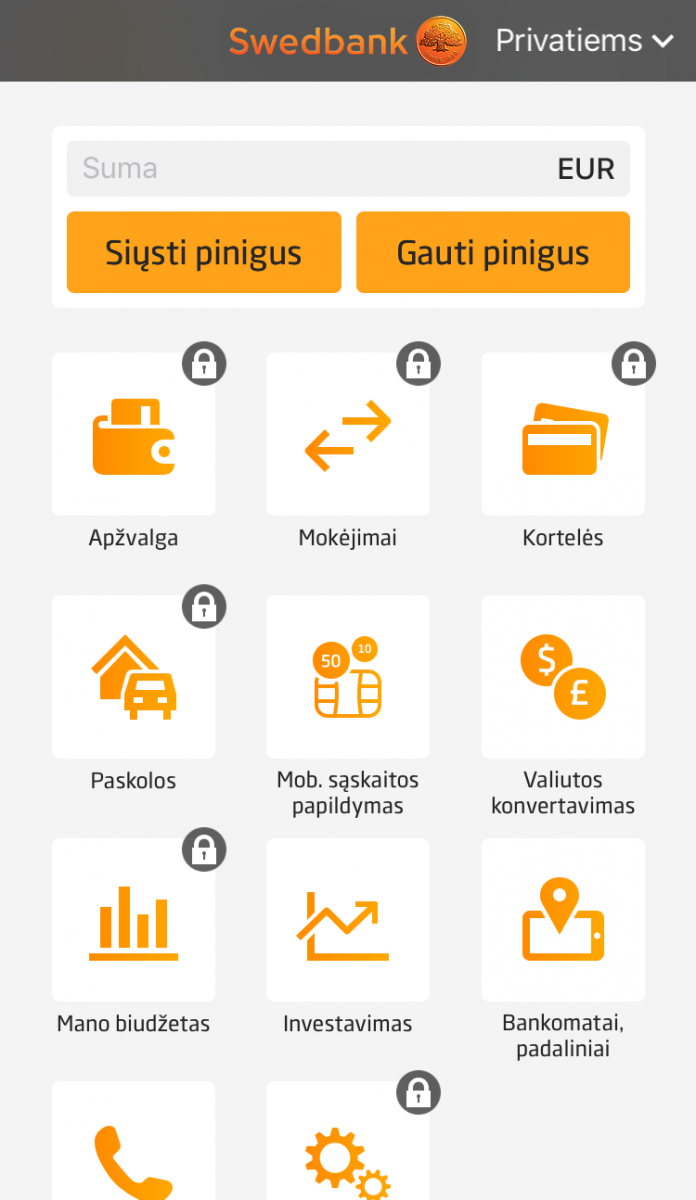
\includegraphics[scale=0.4]{mobileApp.png}
  \caption{Mygtukai iš mobiliosios aplikacijos}
	\label{fig:mobileApp}
	Nauda: Piktogramos visiems labiau suprantamos, lengviau skaitomos, jų pagalba norimus puslapius galima rasti greičiau.
\end{figure}
\begin{figure}[!htb]
  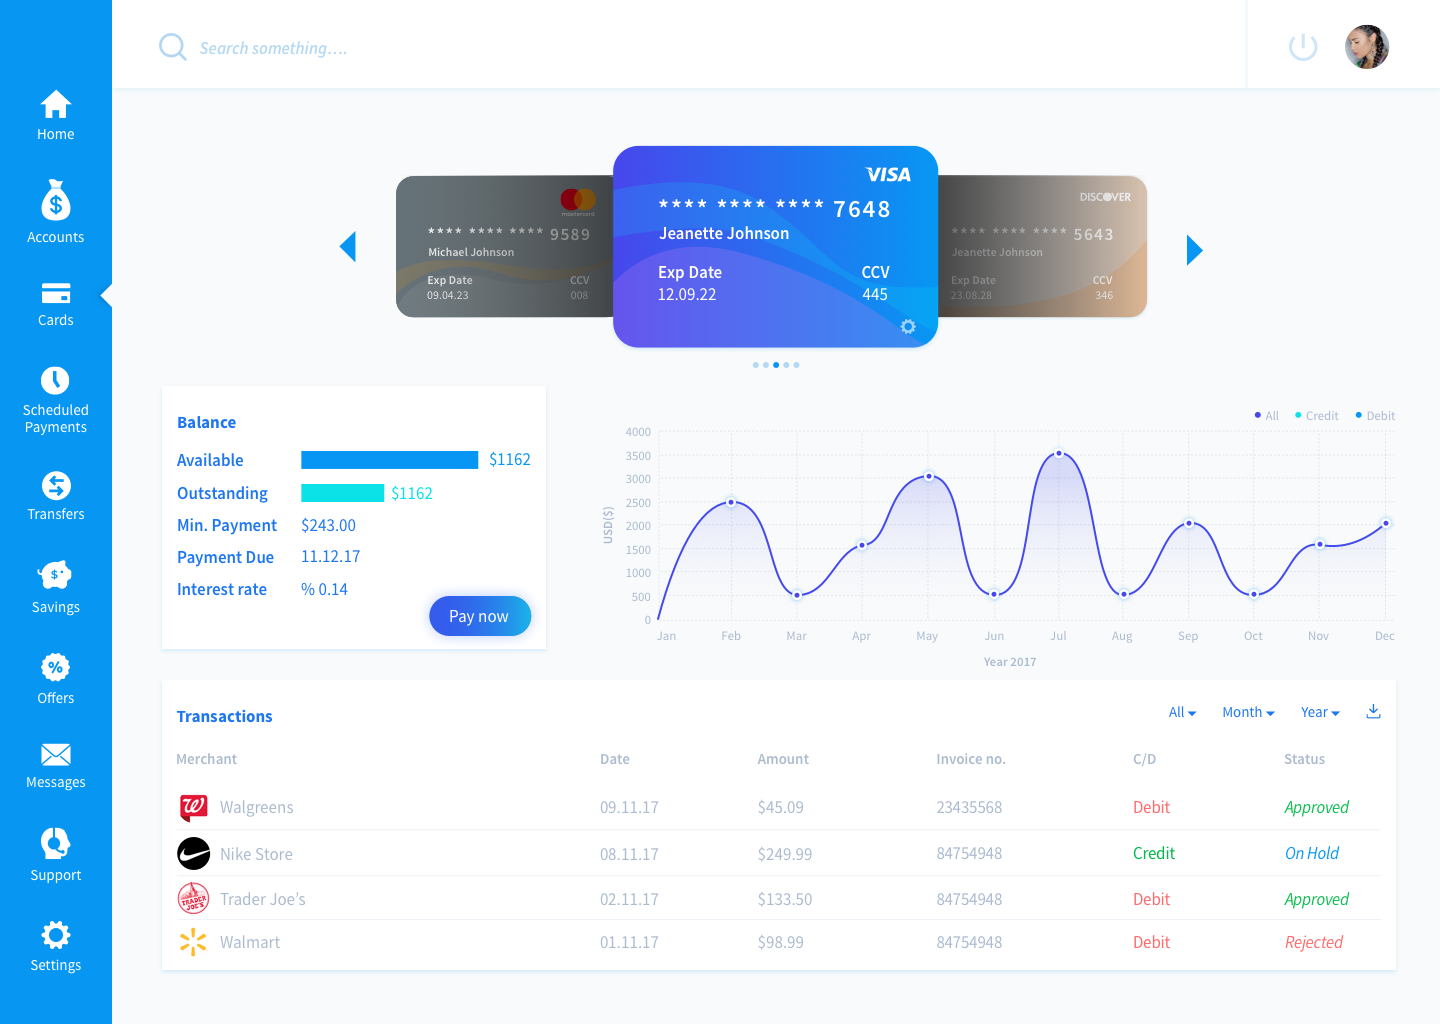
\includegraphics[width=\linewidth]{iconPlacement.png}
  \caption{Mygtukų išdėstymas svetainėje}
	\label{fig:iconPlacement}
	Nauda: Vartotojui aiškus meniu, greitas vaikščiojimas tarp puslapių.
\end{figure}
\begin{figure}[!htb]
  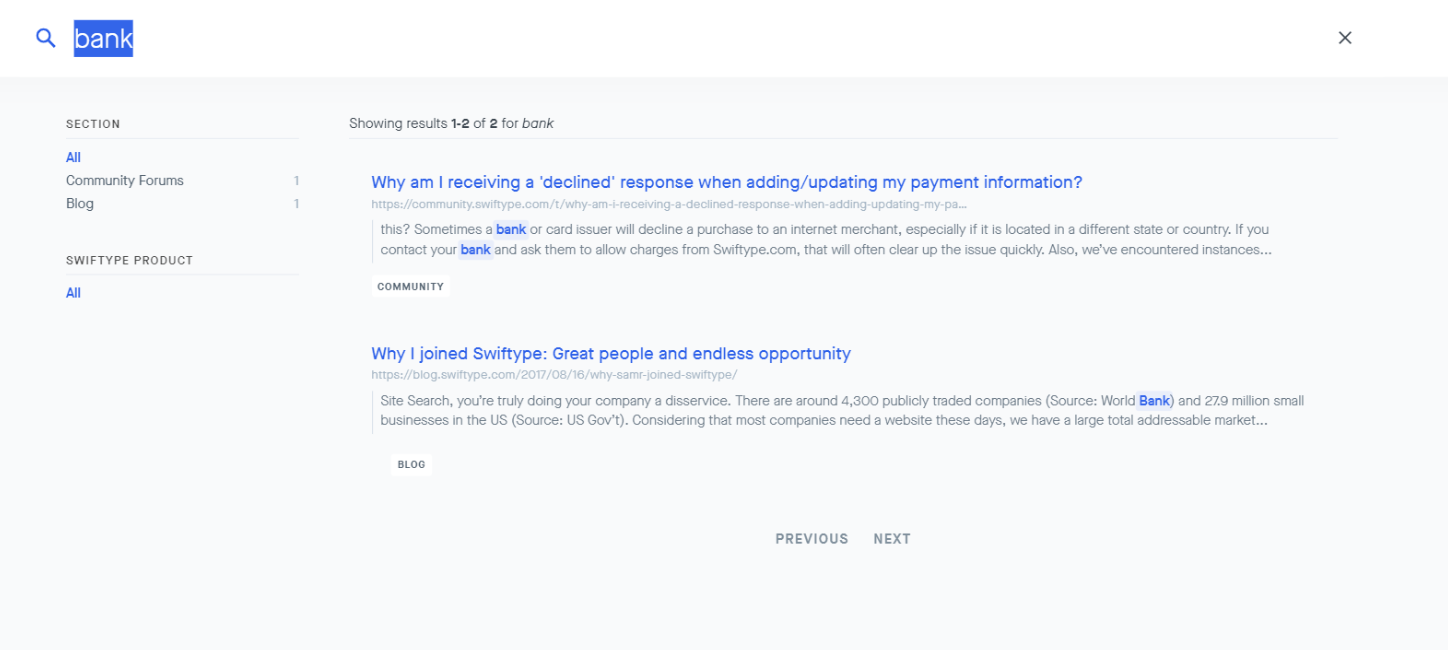
\includegraphics[width=\linewidth]{SearchWindow.png}
  \caption{Informacijos paieškos langas}
	\label{fig:searchWindow}
	Nauda: Vendant tekstą ieškoma po kiekvieno įvesto simbolio, galima filtruoti pagal skirtingas grupes.
\end{figure}
\section{Terminų žodynėlis(maybe)}

\end{document}
